% #########################################################################################
% #########################################################################################
% #########################################################################################
\section{Exercise design}
\label{sec:exercise}
% -----------------------------------------------------------------------------------------
\subsection{Description of the tested functionality}

The present work focuses on the impact of using a \gls{FLM} or a \gls{FF}
approach. 

A \gls{FLM} approach consists to adapt the fresh fuel composition according to
the reactor requirements and the available material isotopic compositions. A
\gls{FLM} connects the fresh fuel composition to the available materials,
regardless to the complexity of the model. For instance, the fissile fraction is
calculated from the fissile stock quality in order to reach the required burn-up
of the reactor. A \gls{FLM} could be based on neural network, Plutonium
equivalence model, analytic functions, built-in depletion, etc. A \gls{FLM} is
usually built from physics constraints and reactor physics calculations. 

A \gls{FF} model consists in using the same constant fissile fraction at each
fresh fuel loading regardless of the isotopic composition of the available
fissile material. Using a \gls{PWR} \gls{MOX} which is always loaded with a
fresh fuel that contains 7\% of plutonium regardless the $^{239}$Pu content is a
\gls{FF} approach. 

The present work aims to quantify the impact of using \gls{FLM} versus \gls{FF}
approach considering this later as the reference, as it should have more physics
refinement. In a fuel cycle simulator, the \gls{FF} approach is the cheapest
method to deal with fresh reprocessed fuel fabrication. Developing \gls{FLM}
may be an important development process requiring time and effort.
Testing the impact of using \gls{FLM} rather than \gls{FF} aims to identify the
study that require \gls{FLM} and the one solvable with \gls{FF}.

\subsection{Output of interest}

Fuel fabrication models can impact fuel cycle simulation in many different ways.
This exercise aims to understand some of their impacts on an overall fuel cycle
calculation. Change in the plutonium content in a \gls{MOX} fuel could impacts
the fuel cycle in 3 majors ways:

\begin{itemize}
    \item global amount of plutonium in the simulation: variation in the
        plutonium content in the \gls{MOX} fuel might lead in an increase of the
        amount of plutonium burnt in the \gls{PWR} reactor and/or a change in the
        breeding/burning ratio in a \gls{SFR} reactor, impacting the overall amount of
        plutonium in the simulation.
    \item location of the plutonium: the amount of plutonium in the \gls{MOX}
        fuel will shift the location of the plutonium from the front-end the
        back-end of the cycle, which could change its availability for other
        uses (deployment of new reactor, fabrication of other fuels\ldots),
    \item variation of the global amount of plutonium relative to the amount
        loaded in the fuel: the breeding/burning ratio of the plutonium might
        change the amount of plutonium in reactor.
\end{itemize}

This might not be exhaustive list of fuel fabrication model impacts on a fuel
cycle studies, but this work will only focus on them and will not consider
potential consequence on the fuel composition change after depletion due to
over/under-estimate the amount of plutonium in the \gls{MOX} fuel.

In order to investigate those impacts across multiple fuel cycle simulation tool
and associated models, the following experience has been designed.

% -----------------------------------------------------------------------------------------
\subsection{Exercise specifications}

The exercise is divided in two independent parts related to the reactor
involved. \gls{PWR} and \gls{SFR} will be considered in this work.

The schematic representation of the fuel cycle is shown on
Figure~\ref{fig:FuelCycle}. The simulation includes a infinite (enough to build
stream of materials, one plutonium stream and one depleted uranium stream. Both
stream feed a fuel fabrication plant which build the MOX fuel for the reactor
(\gls{PWR}  or \gls{SFR}) according the its technical requirements. The reactor
spent fuel is sent away to a storage or to the waste and not considered in
this work.

\begin{figure}[h]
    \begin{center}
        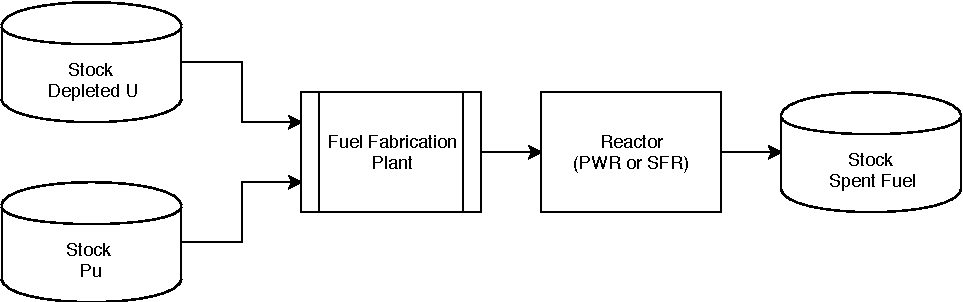
\includegraphics[width = 0.99\textwidth]{FIG/FuelCycleDiagram.pdf}
        \caption{Schematic representation of the simulated fuel cycle facilities.}
        \label{fig:FuelCycle}
    \end{center}
\end{figure}

The simulation last one single the reactor cycle.  At t = 0, the fabrication
plant produces the fresh fuel according to reactor requirements. To avoid
radioactive decay, the fabrication process and the reactor fuel loading are
simultaneous and instantaneous. The MOX-fuel stays in the reactor for a complete
cycle (it reaches it designed \gls{BU} and is then send to the back-end storage.


As it is expected that, for a set reactor, the MOX-fuel plutonium content should depend on the
plutonium isotopic composition, a large rage of plutonium isotopic composition
have been considered, allowing to highlight the different between \gls{FLM} and
\gls{FF} modeling.

Moreover the defined isotopic space as been designed to cover a wide range of
fuel history: a CANDU fuel with low discharge burn-up (high fissile
fraction~\cite{Guillemin_2010}), \gls{PWR} multi-recycled MOX fuel (high even
isotopes fraction in the plutonium~\cite{Courtin_2016}), long cooling time (low
$^{241}$Pu fraction). Therefore, the conclusion of this work is not transposable
to a study where a only narrow plutonium isotopic space is encountered, in this
case a \gls{FF} model would probably be enough. The Table~\ref{tab:PuVector}
presents plutonium isotopic space covered in this work.

\begin{table}[h]
\centering
\begin{tabular}{ |l|l|l| }
  \hline
  Isotope & Min. Mass Fr. (wgt. \%) & Max. Mass Fr. (wgt. \%) \\
  \hline
  Pu-238/TRU & 0  & 10 \\
  \hline
  Pu-239/TRU & 25 & 90 \\
  \hline
  Pu-240/TRU & 10 & 40 \\
  \hline
  Pu-241/TRU & 0  & 25 \\
  \hline
  Pu-242/TRU & 0  & 30 \\
  \hline
  Am-241/TRU & 0  & 10 \\
  \hline
\end{tabular}
\label{tab:PuVector}
\caption{Minimum and maximum mass fraction in weight \% for plutonium vector at
        reactor beginning of cycle used in the framework of this work}
\end{table}

% -----------------------------------------------------------------------------------------
\subsection{Problem-solving methodology}

In order to investigate the influence of using a \gls{FLM} rather than a
\gls{FF} model on fuel cycle simulations, the following experiment have been
designed. Following the FIT project principle, no inter-code comparison will be
done. For each simulator used to solve this problem, fuel models will be
compared within the same simulator, allowing to evaluate difference between two
almost identical simulation: same simulator, reactor description, depletion
algorithm, \ldots The only difference being the method used to build the fresh fuel.

The experiment consists in running a small fuel cycle calculation according to
specifications defined above. We use a method that we call "Wide Parametric
Sweep" method. The principle is to randomly populate the pre-defined isotopic
space (see in the Table~\ref{tab:PuVector}. For each random plutonium
composition the simulation will be ran twice, once using the \gls{FF} model,
i.e. the fraction of plutonium in the fuel is fixed regardless to its isotopic
composition, and once with the \gls{FLM} model adapting its fraction in the fuel
accordingly to its isotopic composition. 

Each code produces for each reactor, \gls{PWR} and \gls{SFR}, two sets of output
data representing \gls{FLM} and \gls{FF} runs. For each case, the output of
interest are the mass of plutonium at \gls{BOC} $M_{Pu}^{BOC}$ and \gls{EOC}
$M_{Pu}^{BOC}$ and the plutonium fraction $\lambda_{\mathrm{Pu}}^{BOC}$ at
\gls{BOC}. Future works will be dedicated to extend the range of output, to
plutonium isotopic composition or minor actinides production. 

In order to measure the influence of using a \gls{FF} versus \gls{FLM} on the
global amount of plutonium in the simulation, the location of the plutonium and
the speed of variation of the plutonium inventory, three estimators have been
defined.


\subsection{Estimators\label{subsec:estimator}}

From output data produced by the different simulators, three estimators have
been design to measure the impact of using a \gls{FF} model over a \gls{FLM}.
Inside a fuel cycle, two scales of effect can dissociated the global effect impacting
the overall simulation, such as total amount of some elements in the simulations
(plutonium, minor actinides\ldots) and the local effect corresponding to the
amount of those element in a specific facility or storage. While global effects
are necessary associated with one or multi local effects, the local effects do
not necessary have a global impact, as an other local effect can compensate it.


\subsubsection{Estimator 1}

The first estimator aims to measure the difference on the plutonium enrichment
in the \gls{MOX} fuel between the \gls{FLM} and \gls{FF}. This estimator directly
impacts the amount of plutonium present in the back-end part of the fuel cycle
and is then a local estimator. The estimator 1 has been defined as:

\begin{equation}
    \delta{\lambda}(i) =
        \frac{\left(\lambda_{\mathrm{Pu}}^{BOC}(i)\right)_{FML}
              - \left(\lambda_{\mathrm{Pu}}^{BOC}(i)\right)_{FF}}
              {\left(\lambda_{\mathrm{Pu}}^{BOC}(i)\right)_{FF}},
\end{equation}

where $\lambda_i$ represents the fraction of plutonium at \gls{BOC} or at
\gls{EOC} for the plutonium composition $i$ for the \gls{FLM} or the \gls{FF}.
The higher the estimator 1 is, the higher the plutonium fraction at \gls{BOC} is
for the \gls{FLM} compared to \gls{FF}. This estimator is used in the case of
\gls{PWR} and \gls{SFR} analysis.

\subsubsection{Estimator 2}

The second estimator aims to estimate the relative speed of plutonium
consumption in the reactor between the \gls{FLM} and the \gls{FF} approach. The
estimator 2 is defined as:

\begin{equation}
    \delta{\frac{\Delta M}{M}}(i) =
        \frac{\left(\frac{\Delta M}{M}(i)\right)_{FML}
              - \left(\frac{\Delta M}{M}(i)\right)_{FF}}
             {\left(\frac{\Delta M}{M}(i)\right)_{FF}},
\end{equation}
where $\frac{\Delta M}{M}_{i}$ is defined as:
\begin{equation}
    \frac{\Delta M}{M}(i) = \frac{M_{Pu}^{BOC}(i) -
    M_{Pu}^{EOC}(i)}{M_{Pu}^{BOC}(i)}
\end{equation}

Estimator 2 represents a global effect since the plutonium consumption speed has
an impact on total plutonium mass. This estimator is suitable for reactor
simulations characterized by plutonium decrease and is used for \gls{PWR} analysis.

\subsubsection{Estimator 2b}

The estimator 2 can tend toward infinity if reactor is iso-breeder. To avoid
such a behavior, a variation of it, the estimator 2b, has been defined as following : 

\begin{equation}
    \delta \frac{\Delta M}{M}(Pu_i) = \frac{\Delta M}{M}(Pu_i)_{FLM} - \frac{\Delta M}{M}(Pu_i)_{FF}
\end{equation}

Estimator 2b measures a global effect and will be used for \gls{SFR} results.

\subsubsection{Estimator 3}

The third estimator shows the absolute speed of plutonium consumption in the
reactor between the \gls{FLM} and the \gls{FF} approach and is defined as
following :

\begin{equation}
    \delta{\frac{\Delta M}{T}}(i) =
        \frac{\left(\frac{\Delta M}{T}(i)\right)_{FML}
              - \left(\frac{\Delta M}{T}(i)\right)_{FF}}
             {\left(\frac{\Delta M}{T}(i)\right)_{FF}},
\end{equation}
where $\frac{\Delta M}{T}_{i}$ is defined as:
\begin{equation}
    \frac{\Delta M}{T}(i) = \frac{M_{Pu}^{BOC}(i) -
    M_{Pu}^{EOC}(i)}{T}
\end{equation}

Estimator 3 characterizes a global effect and is used in the case of \gls{PWR}
simulations analysis.

